
\documentclass[12pt]{article}
\usepackage{geometry}
\geometry{A4}
\usepackage{graphicx}
\usepackage{amssymb}
\usepackage{amsmath}
\usepackage{algorithm}
\usepackage{algpseudocode}
\usepackage{caption}
\usepackage{indentfirst}
\algnewcommand\algorithmicswitch{\textbf{switch}}
\algnewcommand\algorithmiccase{\textbf{case}}
\algdef{SE}[SWITCH]{Switch}{EndSwitch}[1]{\algorithmicswitch\ #1\ \algorithmicdo}{\algorithmicend\ \algorithmicswitch}%
\algdef{SE}[CASE]{Case}{EndCase}[1]{\algorithmiccase\ #1}{\algorithmicend\ \algorithmiccase}%
\algtext*{EndSwitch}%
\algtext*{EndCase}%

\DeclareCaptionFormat{algor}{%
  \hrulefill\par\offinterlineskip\vskip1pt%
    \textbf{#1#2}#3\offinterlineskip\hrulefill}
\DeclareCaptionStyle{algori}{singlelinecheck=off,format=algor,labelsep=space}
\captionsetup[algorithm]{style=algori}

\usepackage{fontspec,xltxtra,xunicode}
\defaultfontfeatures{Mapping=tex-text}


\title{ICSI403: Assignment 1}
\author{Huang Kaisheng <2020215138@stu.cqupt.edu.cn>}
\date{\today}

\begin{document}
\maketitle
\newpage
\tableofcontents
\newpage

\section{Prob. 1}

Illustration:

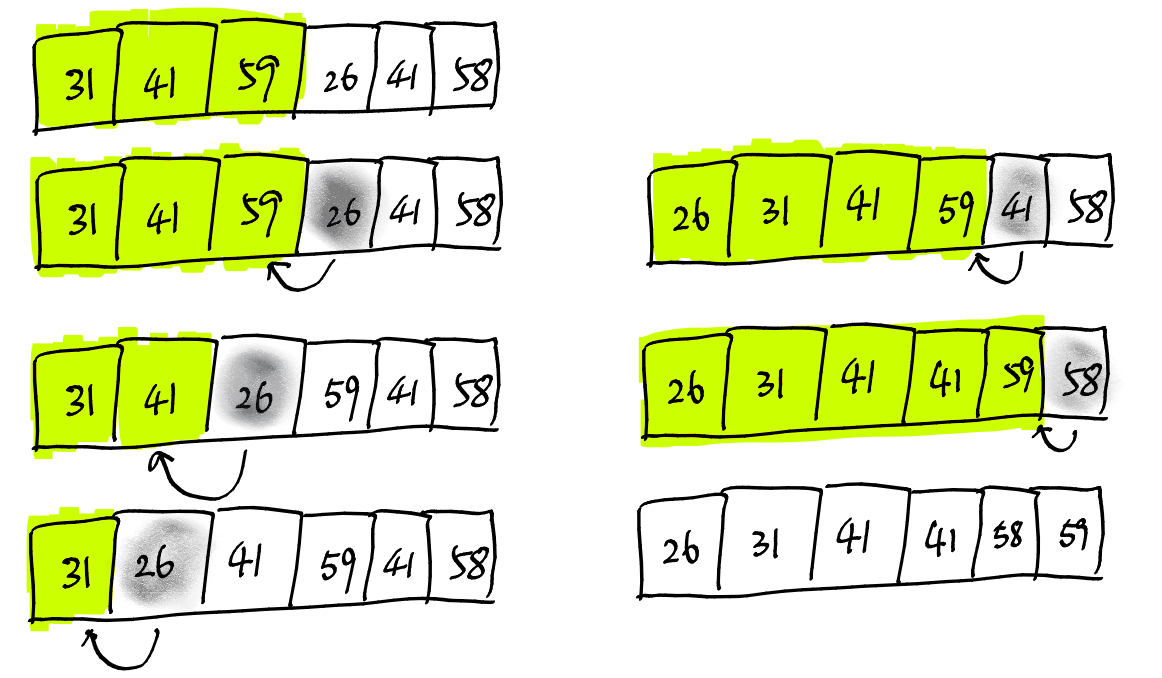
\includegraphics[Illustration]{pics/as1prob1.1.png}

\begin{center}
\captionof{algorithm}{Non-decreasing order insertion sort}
\begin{algorithmic}[1]
    \For {$j \gets 2$ to $A$.length}
        \State {key \gets $A_j$}
        \State {$i \gets j - 1$}
        \While {$i > 0$ and $A_i \leq $ key}    \Comment{Judge if $A_i$ is less equal than key}
            \State {$A_{i+1} \gets A_i$}
            \State {$i \gets i - 1$}
        \EndWhile
        \State {$A_{i + 1} = $ key}
    \EndFor
\end{algorithmic}
\end{center}

\newpage
\section{Prob. 2}

\begin{center}
\captionof{algorithm}{Compute the sum of $a$ and $b$ in binary form}
\begin{algorithmic}[1]
    \Procedure{BinarySum}{$a, b$: BitArray}
        \State $s \gets [\mathrm{Empty BitArray}], c \gets 0$
        \If {$a$.length < $b$.length}
            \State $(a, b) \gets (b, a)$
        \EndIf
        \For {$i \gets 0$ to $b.\mathrm{length} - 1$}
            \State $s_i \gets (a_i \oplus b_i \oplus c)$
            \State $c \gets (a_i \land b_i) \lor (a_i \land c) \lor (b_i \land c)$
        \EndFor
        \For {$i \gets b.\mathrm{length}$ to $a$.length}
            \State $s_i \gets a_i \oplus c$
            \State $c \gets a_i \land c$
        \EndFor
        \State $s_{a.\mathrm{length}} \gets c$
        \State \Return $s$
    \EndProcedure
\end{algorithmic}
\end{center}

Illustration of $a = (1110)_2$ and $b = (1011)_2$:

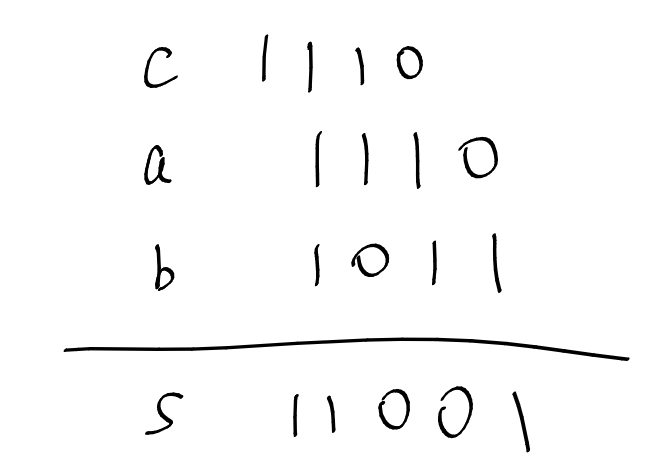
\includegraphics[Illustration]{pics/as2prob2.1.png}

\section{Prob. 3}

\subsection{$(n^2+8)(n+1)$}
$$
\begin{aligned}
\Theta((n^2+8)(n+1)) &= \Theta(n^3 + n^2 + 8n + 8) \\
&= \Theta(n^3)
\end{aligned}
$$

\subsection{$(n\log n + n^2)(n^3+2)$}
$$
\begin{aligned}
\Theta((n\log n + n^2)(n^3+2)) &= \Theta(n^3 \log n + n^5 + 2n \log n + 2n^2) \\
&= \Theta(n^5)
\end{aligned}
$$

\subsection{$(n!+2^n)(n^3+\log{(n^2+1)})$}
First, $n! = n(n-1)(n-2)\cdots 1$, whose $\Theta$-notation should be $\Theta(n^{n-1})$.


$$
\begin{aligned}
\Theta((n!+2^n)(n^3+\log{(n^2+1)})) &= \Theta((n^{n-1}+2^n)(n^3+\log{(n^2+1)})) \\
&= \Theta(n^{n+2} + n^{3}\cdot 2^n + n^{n-1} \log{(n^2+1)} + 2^n \log{(n^2+1)}) \\
&= \Theta(n^{n+2})
\end{aligned}
$$

\section{Prob. 4}
\subsection{(1)}
In the problem we have already proved termination, so we need to prove the initialization and maintenance part.

\subsection{(2)}
The loop invariant is $j \geq i + 1$. For the inner loop, it iterates backward and tries to find a larger value than the value visited in outer loop, and then swaps them. After each iteration of the inner loop (with index $j$), there must be $A_i \leq A_j$.

\subsection{(3)}
Proof:

Initialization: Prior to the 1st iteration, the array $A$ is a trivial array that should be sorted, and the first subarray $\{A_1\}$ is sorted.

Maintenance: For outer loop, it iterates forward (with index $i$) and visits each element of the array. After each iteration of outer loop, there must be $A_i \leq A_k (\forall k > i)$, thus the subarray $\{A_1,A_2,\cdots,A_{i-1}\}$ is sorted.

Termination: The outer loop stops when $i = A.\mathrm{length}$. All subarrays are sorted, so the entire array is sorted.

\section{Prob. 5}

\subsection{(1) Devising}

\begin{center}
\captionof{algorithm}{Locates all occurrences of an integer $x$ in the non-ascending sorted list}
\begin{algorithmic}[1]
    \Procedure{locate}{$x$: integer, $A$: integer[]}
        \State {indexes $\gets \mathrm{[Empty Array]}$}
        \Procedure{locateRecursion}{$l, r$: integer}
            \State {mid \gets $\lfloor \frac{l + r}{2} \rfloor$}
            \If {$A_\mathrm{mid} > x$}
                \State \Return {locateRecursion($l$, mid)}
            \ElsIf {$A_\mathrm{mid} < x$}
                \State \Return {locateRecursion(mid, $r$)}
            \Else
                \For {$i \gets \mathrm{mid}$ \mathrmbf{down and} $A_i = x$}
                    \State {indexes:push($i$)}
                \EndFor
                \For {$i \gets \mathrm{mid} + 1$ \mathrmbf{up and} $A_i = x$}
                    \State {indexes:push($i$)}
                \EndFor
            \EndIf
        \EndProcedure
        \State {locateRecursion(0, $A$.length)}
        \State \Return {indexes}
    \EndProcedure
\end{algorithmic}
\end{center}

\subsection{(2) Estimate the number of comparisons used}

We use binary search to find the integer in a non-ascending sorted list. When we find one occurrence, we expand to its left neighbors and right neighbors.

So the estimation should be $\log n + m$, where $n$ is the length of the list, $m$ is the occurrences of the target integer. 

\section{Prob. 6}

To prove that $n^3 - 91n^2 - 7n - 14 = \Omega(n^3)$, we need to show that there exist positive constants $c$ and $n_0$ such that for all $n \geq n_0$, we have:

$$n^3 - 91n^2 - 7n - 14 \geq cn^3$$

First, we can simplify the left-hand side of the inequality as follows:

$$n^3 - 91n^2 - 7n - 14 \geq n^3 - \frac{91n^3}{100} - \frac{n^3}{100} - \frac{n^3}{100} \geq \frac{n^3}{2}$$

where we have used the fact that $n^3/100 \leq n^2$ for sufficiently large $n$. Therefore, we have:

$$n^3 - 91n^2 - 7n - 14 \geq \frac{n^3}{2}$$

To satisfy the inequality, we can choose $c=\frac{1}{2}$ and $n_0=1$. Then, for all $n \geq n_0=1$, we have:

$$n^3 - 91n^2 - 7n - 14 \geq \frac{n^3}{2} \geq cn^3$$

Thus, we have shown that $n^3 - 91n^2 - 7n - 14 = \Omega(n^3)$ with $c=\frac{1}{2}$ and $n_0=1$.

\section{Prob. 7}
To prove that $27n^2 + 18n = \Theta(0.5n^2 – 100)$, we need to show that there exist positive constants $c_1$, $c_2$, and $n_0$ such that for all $n \geq n_0$:

$$c_1(0.5n^2 - 100) \leq 27n^2 + 18n \leq c_2(0.5n^2 - 100)$$

Let's start with the lower bound:

\begin{align*}
c_1(0.5n^2 - 100) &\leq 27n^2 + 18n \\
0.5c_1n^2 - 100c_1 &\leq 27n^2 + 18n \\
0.5c_1n^2 &\leq 27n^2 + 18n + 100c_1 \\
c_1 &\leq \frac{54n + 36 + \frac{200c_1}{n^2}}{n^2}
\end{align*}

For any value of $n$, we can choose $c_1 = \frac{n^2}{200}$, which gives us:

$$c_1 = \frac{n^2}{200} \leq \frac{54n + 36 + 200\cdot\frac{n^2}{n^2}}{n^2} = \frac{54n + 236}{n^2}$$

If we choose $n_0 = 1$ (the smallest possible value of $n$), then for all $n \geq n_0$, we have:

$$\frac{n^2}{200} \leq \frac{54n + 236}{n^2}$$

Next, let's move on to the upper bound:

\begin{align*}
27n^2 + 18n &\leq c_2(0.5n^2 - 100) \\
27n^2 + 18n &\leq 0.5c_2n^2 - 100c_2 \\
0 &\leq 0.5c_2n^2 - 27n^2 - 18n - 100c_2 \\
0 &\leq 0.5c_2n^2 - n(27n + 18) - 100c_2 \\
\end{align*}

Using the quadratic formula, we get:

$$n \geq \frac{27 + \sqrt{729 + 200c_2}}{2}$$

We can choose $c_2 = 28$ and $n_0 = 10$ (for simplicity) and show that the upper bound holds for all $n \geq n_0$:

\begin{align*}
27n^2 + 18n &\leq 28(0.5n^2 - 100) \\
27n^2 + 18n &\leq 14n^2 - 2800 \\
13n^2 - 18n &\leq -2800 \\
n^2 - \frac{18}{13}n &\leq -\frac{2800}{13} \\
\end{align*}

Using the completing the square method, we get:

$$\left(n - \frac{9}{13}\right)^2 \leq \frac{29569}{169}$$

Therefore, for all $n \geq 10$, we have:

$$n - \frac{9}{13} \leq \sqrt{\frac{29569}{169}} \approx 16.1$$

$$n \leq \frac{9}{13} + \sqrt{\frac{29569}{169}} \approx 16.87$$

Since $n \geq 10$, we can conclude that the upper bound holds for all $n \geq n_0$.

Therefore, we have shown that $27n^2 + 18n = \Theta(0.5n^2 - 100)$ with $c_1 = \frac{n^2}{200}$, $c_2 = 28$, and $n_0 = \max\{1, \frac{27 + \sqrt{729 + 200c_2}}{2}, 10\} \approx 17$.

\section{Prob. 8}

\begin{center}
\captionof{algorithm}{Strassen algorithm}
\begin{algorithmic}[1]
    \Procedure{Strassen}{$A,B$: Matrix with $2^k$ dimensions}
    \If{$n = 1$}
    \State \Return $A \cdot B$
    \EndIf
    \State Partition $A$ and $B$ into $2 \times 2$ matrices:
    \State $A = \begin{bmatrix} A_{11} & A_{12} \\ A_{21} & A_{22} \end{bmatrix}$, $B = \begin{bmatrix} B_{11} & B_{12} \\ B_{21} & B_{22} \end{bmatrix}$
    \State $P_1 = \mathrm{Strassen}(A_{11}, B_{12} - B_{22})$ \Comment{Compute 7 products recursively}
    \State $P_2 = \mathrm{Strassen}(A_{11} + A_{12}, B_{22})$
    \State $P_3 = \mathrm{Strassen}(A_{21} + A_{22}, B_{11})$
    \State $P_4 = \mathrm{Strassen}(A_{22}, B_{21} - B_{11})$
    \State $P_5 = \mathrm{Strassen}(A_{11} + A_{22}, B_{11} + B_{22})$
    \State $P_6 = \mathrm{Strassen}(A_{12} - A_{22}, B_{21} + B_{22})$
    \State $P_7 = \mathrm{Strassen}(A_{11} - A_{21}, B_{11} + B_{12})$
    \State $C_{11} = P_5 + P_4 - P_2 + P_6$ \Comment{Compute the four quadrants of the product}
    \State $C_{12} = P_1 + P_2$
    \State $C_{21} = P_3 + P_4$
    \State $C_{22} = P_5 + P_1 - P_3 - P_7$
    \State \Return $\begin{bmatrix} C_{11} & C_{12} \\ C_{21} & C_{22} \end{bmatrix}$
    \EndProcedure
    \EndProcedure
\end{algorithmic}
\end{center}

For the matrices
$A = \begin{bmatrix}
2 & 1 \\
3 & 2 \\
\end{bmatrix}, B = \begin{bmatrix}
0 & 4 \\
1 & 3 \\
\end{bmatrix}$, the base case of the recursion is when the size of the submatrices is $1 \times 1$, in which case we simply multiply the corresponding elements. 

$$A_{11}=2,A_{12}=1,A_{21}=3,A_{22}=2,$$
$$B_{11}=0,B_{12}=4,B_{21}=1,B_{22}=3.$$

So, 
$$A_{11}B_{11} = 2 \cdot 0 = 0, \quad A_{12}B_{21} = 1 \cdot 1 = 1, $$
$$A_{11}B_{12} = 2 \cdot 4 = 8, \quad A_{12}B_{22} = 1 \cdot 3 = 3, $$
$$A_{21}B_{11} = 3 \cdot 0 = 0, \quad A_{22}B_{21} = 2 \cdot 1 = 2, $$
$$A_{21}B_{12} = 3 \cdot 4 = 12, \quad A_{22}B_{22} = 2 \cdot 3 = 6.$$

The answer:
$$
AB = \begin{bmatrix}
0 + 1 & 8 + 3 \\
0 + 2 & 12 + 6
\end{bmatrix} = \begin{bmatrix}
1 & 11 \\
2 & 18
\end{bmatrix}.$$

\section{Prob. 9}

Guess the final form is $T(n) = an^2 + bn + c$,

Substitute:
\begin{align*}
T(n) &= T(n-1) + n \\
an^2 + bn + c &= a(n-1)^2 + b(n-1) + c + n \\
&= an^2 + (b - 2a)n + (a - b + c)
\end{align*}

Make all coefficients equal:

\begin{align*}
a &= a \\
b - 2a &= 0 \\
a - b + c &= 0
\end{align*}

With the results above, we can get $T(n) = an^2 + 2an + 3a$.

Prove that $T(n) \leq cn^2$ for some constant $c$ and for all $n$ greater than some minimum value $n_0$.

Let $c = 4a$. Then, for $n \geq 2$, we have:

\begin{align*}
T(n) &= an^2 + 2an + 3a \\
&\leq an^2 + 2an^2 + 3an^2 &(n \geq 2) \\
&= 6an^2 \\
&= cn^2
\end{align*}

Thus, we have shown that $T(n) = \mathrm{O}(n^2)$, since we have found constants $c$ and $n_0$ such that $T(n) \leq cn^2$ for all $n \geq n_0$.

\section{Prob. 10}

To determine a good asymptotic upper bound on the recurrence $T(n) = 4T(\frac{n}{2} + 2) + n$, we will use a recursion tree. At each level of the tree, we will multiply the cost of the recursive call by the number of recursive calls at that level.

\begin{align*}
T(n) &= 4T(\frac{n}{2} + 2) + n \\
&= 4(4T(\frac{n}{4} + 2) + \frac{n}{2} + 4) + n \\
&= 16T(\frac{n}{4} + 2) + 5n + 16 \\
&= 16(4T(\frac{n}{8} + 2) + \frac{n}{4} + 4) + 5n + 16 \\
&= 64T(\frac{n}{8} + 2) + 21n + 64 \\
&\vdots \\
&= 4^kT(\frac{n}{2^k} + 2) + (4^k - 1)n + 4^k\cdot 2.
\end{align*}

We stop when $\frac{n}{2^k} + 2 = 1$, which gives $k = \log_2 (\frac{n}{2} - 2)$. Substituting this value of $k$ back into the expression for $T(n)$, we get:

\begin{align*}
T(n) &= 4^{\log_2 (\frac{n}{2} - 2)} T(1) + (4^{\log_2 (\frac{n}{2} - 2)} - 1)n + 4^{\log_2 (\frac{n}{2} - 2)}\cdot 2 \\
&= (\frac{n}{2} - 2)^2 + (n-2) + 2(\frac{n}{2} - 2) \\
&= (\frac{n}{2})^2 - 3n + 4.
\end{align*}

Therefore, we have determined that $T(n) = \mathrm{O}(n^2)$.

Suppose $T(k) \leq ck^2$ for all $k < n$, where $c$ is a constant. Then:

\begin{align*}
T(n) &= 4T(\frac{n}{2} + 2) + n \\
&\leq 4c(\frac{n}{2} + 2)^2 + n \\
&= cn^2 + 8cn + 16c + n \\
&= cn^2 + (8c + 1)n + 16c.
\end{align*}

If we choose $c$ such that $8c + 1 \leq 0$, then $T(n) \leq cn^2$ for all $n$, and we have proven that $T(n) = \mathrm{O}(n^2)$.

For example, we can choose $c = 1/8$, which satisfies $8c + 1 = 2 \leq 0$. Therefore, we have verified that $T(n) = \mathrm{O}(n^2)$.

\section{Prob. 11}

Let $T(n) = aT(\frac{n}{b}) + f(n)$.

\subsection{(1) $ T(n) = 2T(\frac{n}{4}) + 1$}

We have $a = 2$, $b = 4$, and $f(n) = 1$. 

Therefore, $f(n) = O(n^{\log_b a - k})$ for any $k > 0$, since $n^{\log_b a - k} = n^{\log_4 2 - k} = n^{\frac{1}{2} - k}$. 

By the master method, we conclude that $T(n) = \Theta(n^{\log_b a}) = \Theta(\sqrt{n})$.

\subsection{(2) $ T(n) = 2T(\frac{n}{4}) + \sqrt{n}$}

We have $a = 2$, $b = 4$, and $f(n) = \sqrt{n}$. 

Therefore, $f(n) = \Theta(n^{\log_b a})$, since $n^{\log_b a} = n^{\log_4 2} = \sqrt{n}$. 

By the master method, we conclude that $T(n) = \Theta(n^{\log_b a} \log n) = \Theta(\sqrt{n} \log n)$.

\end{document}